\documentclass[12pt]{article}

\usepackage{sbc-template}

\usepackage{graphicx,url}

\usepackage[brazil]{babel}   
%\usepackage[latin1]{inputenc}  
\usepackage[utf8]{inputenc}  
% UTF-8 encoding is recommended by ShareLaTex

     
\sloppy

\title{Relatorio da segunda entrega do codigo ``organizador de atividades extras na UFRJ''}

\author{Luiz Henrique Gonçalves Miranda\inst{1} }


\address{Universidade Federal do Rio de Janeiro
  (UFRJ)\\
  -- Rio de Janeiro -- RJ -- Brazil
  \email{luizhenrique0706@poli.ufrj.br}
}

\begin{document} 

\maketitle
     
\begin{resumo} 
  O trabalho se trata de uma entrega final da máteria linguagem de programação do segundo semestre do ano de 2018
  O mesmo se trata de complementar a resolução do problema, criando mais features para o mesmo, onde agora possui prazo
  e controle de acesso fisico
\end{resumo}


\section{Informações Gerais}

Se trata de um acressimo do trabalho, que deve ser melhorado, possui apenas a implementação conceitual, por exemplo
a utilização do motor servo e um adc ao inves de um um leitor de digital como o desejado, pela simplicidade.



\section{Problema}

Com a nova obrigatoriedade de mais horas de atividades extras para se conseguir o diploma na UFRJ, se torna mais obvio 
e gritante a necessidade de uma plataforma que facilite as ofertas e divulgação de vagas para os mesmo, além de reunir
documentos e links necessarios para tais atividades serem apreciados pelas multiplas secretarias de cada instituição
principalmente, quando se faz entre instituições diferentes (ex: departamento de Historia, no campus Praia Vermelha 
recebendo documentos de uma extensão realizada na Politecnica), já que por mais que os documentos do siga sejam iguais,
as coordenações que dão parecer, podem ser desconhecidas dos alunos.



\section{Principio da modelagem}
A modelagem inicial, para teste de conceito, alunos que desejam entrar em projetos e coordenadores de projetos, são iguai
e indiferentes em relação ao centro, ou seja, a entidade que possui as informações de centro foi desconsiderada (nela
se dá informações do centro e um pequeno 'about', sem bloqueio ou aviso nenhum além do nome e endereço, ela deveria 
ainda possuir documentos especificos completando os documentos genericos da UFRJ que é dado no 
options-post além disso ela geraria filtragens de vagas necessarias, tanto para quem oferece, quanto para quem procura).


Além disso, a extrapolação do user feita pelo options-user, geraria uma chave conjunta para uma criar os parametros basicos
para os provaveis, e inseridos campos citados:

\subsection{Adminitrador}

Administrador não foi alterado

\subsection{Criadores de oportunidades}

Eles receberam novas responsabilidades, agora devem decidir o dia de encerramento das oportunidades, além disso,
possuem o poder de selecionar os pedidores de vagas que desejam

\subsection{Pedidores de oportunidades}

Agora na hora de se cadastrar, possuem a oportunidade de escrever uma especie de curriculo que será lido pelo criador
da oportunidade desejada


\section{Visual}\label{sec:figs}


\subsection{Novidades dos criadores de oportunidades }

\begin{figure}[ht]
\centering
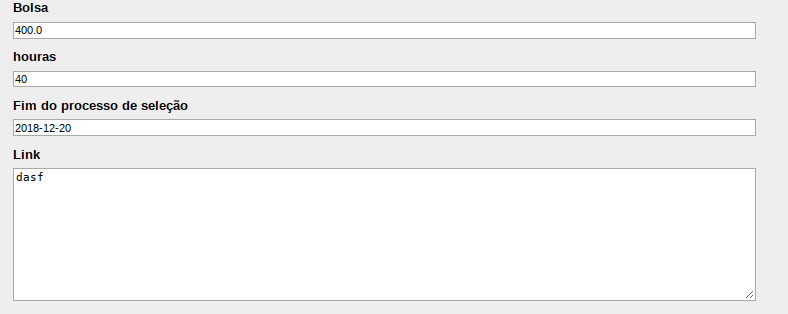
\includegraphics[width=.5\textwidth]{imagens/horarios.png}
\caption{Exemplo de horario, deve respeitar o formato yyyy-mm-dd e ser maior que o dia atual}
\end{figure}

\begin{figure}[ht]
\centering
\includegraphics[width=.5\textwidth]{imagens/seleção.png}
\caption{Exemplo de lista de selecionaveis}
\end{figure}

\begin{figure}[ht]
\centering
\includegraphics[width=.5\textwidth]{imagens/seleção2.png}
\caption{Selecionando o selecionavel}
\end{figure}

\clearpage
\subsection{Novidades dos pedidores de oportunidades}

\begin{figure}[ht]
\centering
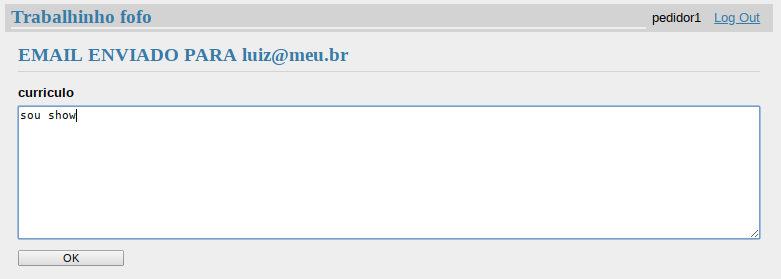
\includegraphics[width=.5\textwidth]{imagens/email.png}
\caption{Exemplo escrevendo o curriculo no email}
\end{figure}

\begin{figure}[ht]
\centering
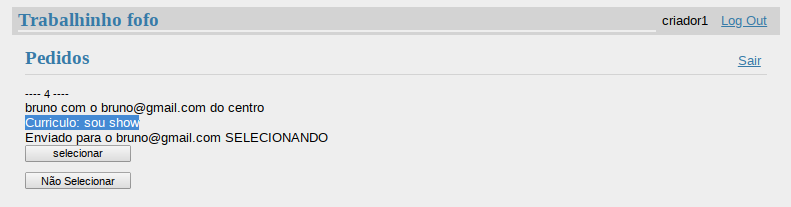
\includegraphics[width=.5\textwidth]{imagens/curriculo.png}
\caption{Como visto realmente aparece o 'curriculo do email'}
\end{figure}


\begin{figure}[ht]
\centering
\includegraphics[width=.5\textwidth]{imagens/seleção2.png}
\caption{Selecionando o selecionavel}
\end{figure}

\clearpage
\subsection{Controle da porta}

\begin{figure}[ht]
\centering
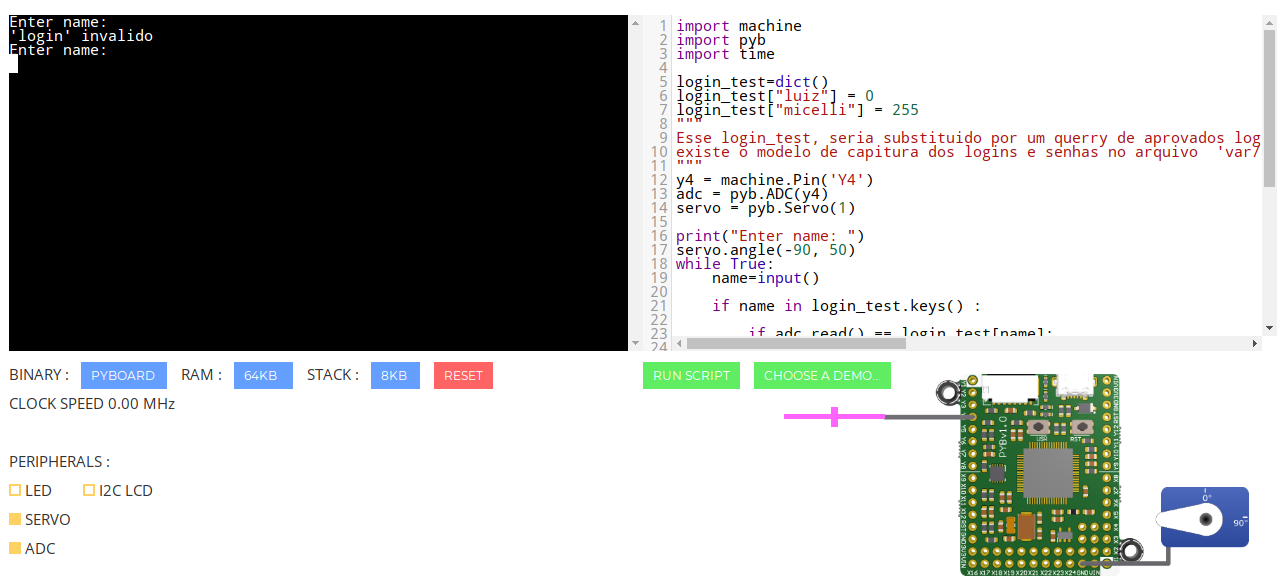
\includegraphics[width=.5\textwidth]{imagens/fechada.png}
\caption{Inicialmente fechada}
\end{figure}

\begin{figure}[ht]
\centering
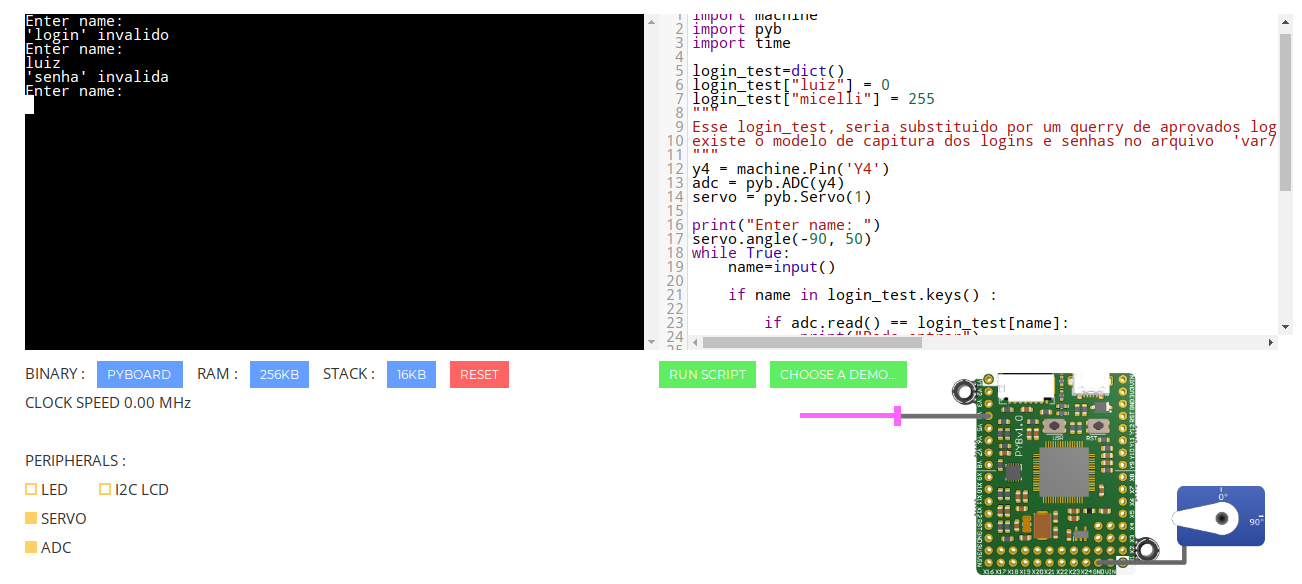
\includegraphics[width=.5\textwidth]{imagens/fechada2.png}
\caption{Se mantem fechada pelo erro de senha ('reparar no adc')}
\end{figure}

\begin{figure}[ht]
\centering
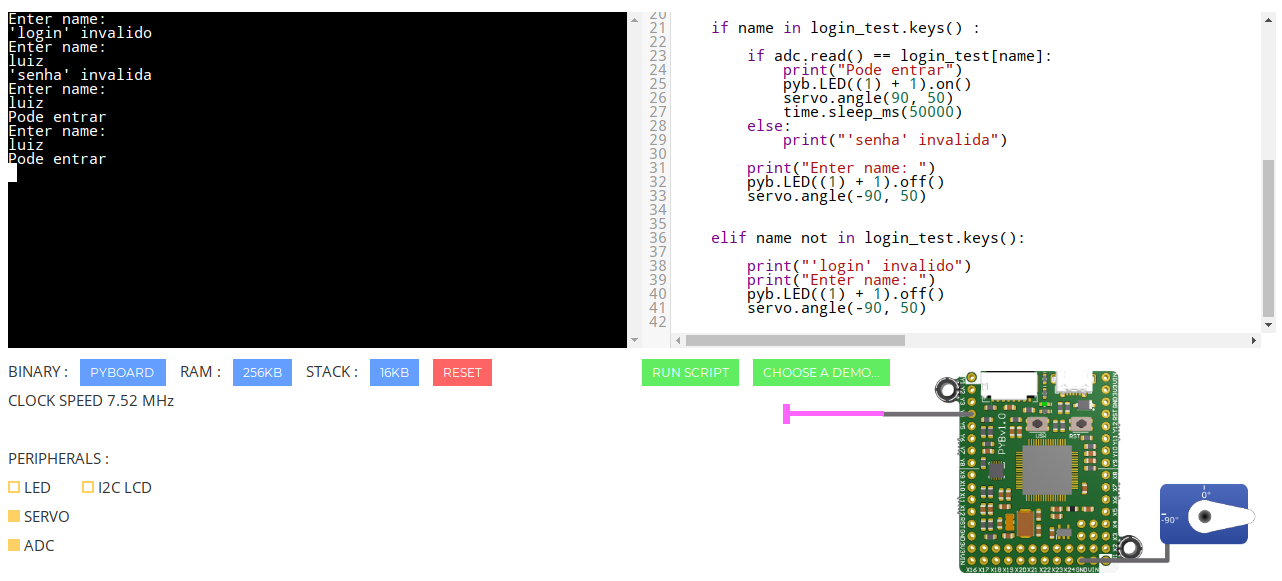
\includegraphics[width=.5\textwidth]{imagens/aberta.png}
\caption{Abre com a senha e login correto ('reparar adc e servo')}
\end{figure}

\begin{figure}[ht]
\centering
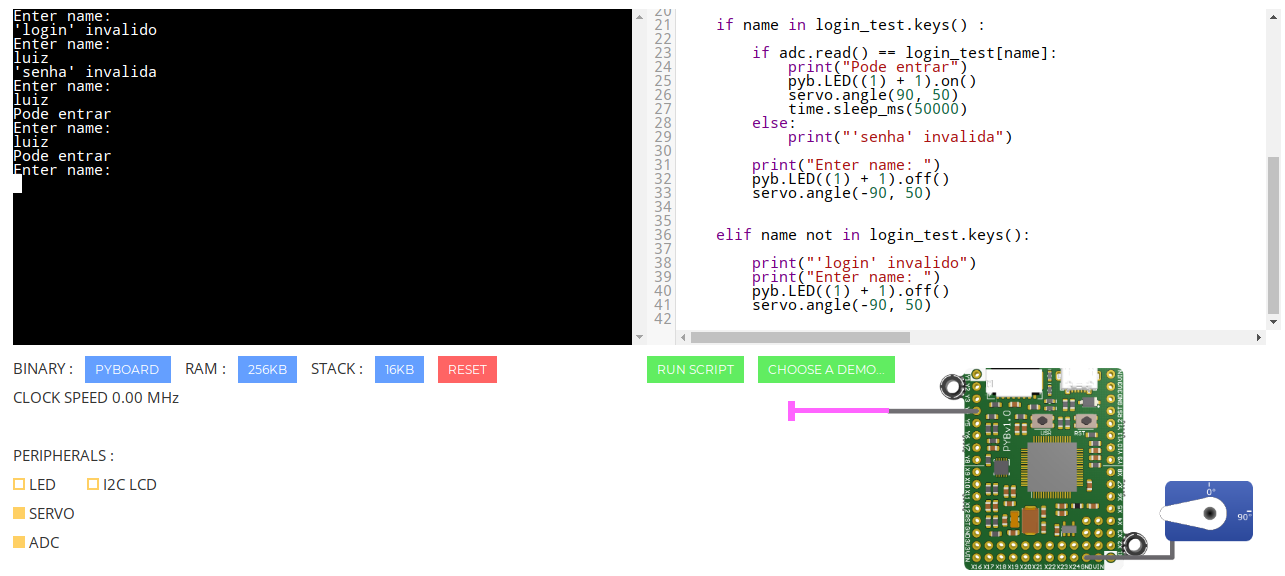
\includegraphics[width=.5\textwidth]{imagens/fechada3.png}
\caption{Volta a fechar ('repare que nada foi escrito de novo no terminal e o servo voltou a posição fechada')}
\end{figure}

\section{Considerações}
Ainda necessita de bastante trabalho e alterações, principalmente no formato de integração da IOT que esta simplista
apenas um arquivo que será carregado, embora funcional, deveria ser pensado uma nova forma de senha e principalmente a
utilização de outro sensor, como dito em outras partes, não deveria ser um simples ADC que funciona como prova de
conceito apenas. Mas que poderia ser melhorado e desenvolvido no futuro.


\section{References}

Curso de Flask

\bibliographystyle{sbc}

\end{document}
